\subsection{Distributed approach with communication}
\label{subsec:ex1comm}

\subsubsection{Model training}
\label{subsubsec:learnedcomm}
An alternative to the previous approach involves the possibility of training a 
new distributed network that exploit a communication protocol between 
agents to decide more reliably the output control.

Using the same data collected in the previous approach we build a model that 
at each timestep takes as input for each robot an array containing the 
response values of the sensors – which can be either \texttt{prox\_values}, 
\texttt{prox\_comm} or \texttt{all\_sensors} – and the message received in 
the previous timestep, communicated by the nearest agents (one on the left 
and one on the right), and produces as output an array of 2 floats, 
corresponding the first one to the control, which, as before, is the speed of 
the wheels, and the second one to the communication, i.e. the message 
transmitted by the robot to the nearest agents.

Also for this purpose, the model is independent of the number of agents in 
the simulations. Instead, in this approach is important to keep track of the 
timesteps order since the input of the network requires the communication 
received in the actual timestep which corresponds to a message transmitted 
in the previous one. 
To do so, a preprocessing is applied to the dataset in order to combine 
consecutive timesteps into a set of sequences. Therefore, we divide each 
simulation in sequences of length $2$, or composed by two consecutive 
timesteps, using a stride of $1$ among them, which contains an ordered 
series of two states for each robot.   

For this model the shape of the input has been transformed from $1 \times 
\mathtt{input\_size}$ to $\mathtt{seq\_length} \times \mathtt{N} \times 
\mathtt{input\_size}$, where \texttt{seq\_length} is fixed at $2$, $N$ is variable 
and \texttt{input\_size} can be $7$ or $14$.

It is important to notice that the communication is not yet in the input since 
it is not contained in the original dataset, instead is treated as a hidden 
variable to be inferred. 
At the beginning of each sequence there are no previous timesteps to 
consider since no messages have been received yet. Therefore, a placeholder 
is randomly initialised, filled with float values in the range $[0, 1]$. 
The size of this array corresponds to the number of agents plus two 
elements, one at the beginning and one at the end of the vector, always set 
to $0$, since they are used to store the fact that the two extreme robots 
never receive messages respectively from the left or from the right. 
The random initialisation of this vector is essential to increase the 
generalization capabilities of the network during its training, showing it 
different starting situations.

Another crucial aspect to consider when using communication is the type of   
updated protocol to choose. As we have already said in section 
\ref{subsec:thymiocomm}, each robot transmits a message every 0.1\gls{s} 
and likewise receives one for each of the sensors. In our case, we expect 
each agent to receive two communications, one for each of its respective 
neighbours. 
With real robots, but also in simulation, what we want to attain is a 
synchronous communication update protocol. Formally, each robot $n$, 
given the observations at time $t$, that correspond to the sensor readings 
$S_n(t)$, and the communications at time $t-1$, in particular $C_{n-1}(t-1)$ 
and $C_{n+1}(t-1)$, calculates the control $V_n(t)$ and the message to 
transmit $C_n(t)$. 
Adopting this policy it is not important to keep track of the order of the 
robots and it is as if the agents operate simultaneously. 
Ideally, the frequency of updates must be lower than that with which the 
robots exchange messages, however it can happen that due to delays or 
noise in the sensor readings the communication of some robots is not 
received or transmitted. In this case, the array is not updated and the last 
message received is keep instead. 

As a consequence, we define a recurrent structure of the communication 
network, shown in Figure \ref{fig:commnet1}. It is composed by two nested 
modules: in the high-level operates the \texttt{CommNet} that handle the 
sensing of all the agents, while in the low-level the \texttt{SingleNet} that 
works on the sensing and the communication received by a single agent in a 
certain timestep, producing as output the control and the communication to 
transmit. 
\begin{figure}[!htb]
	\centering
	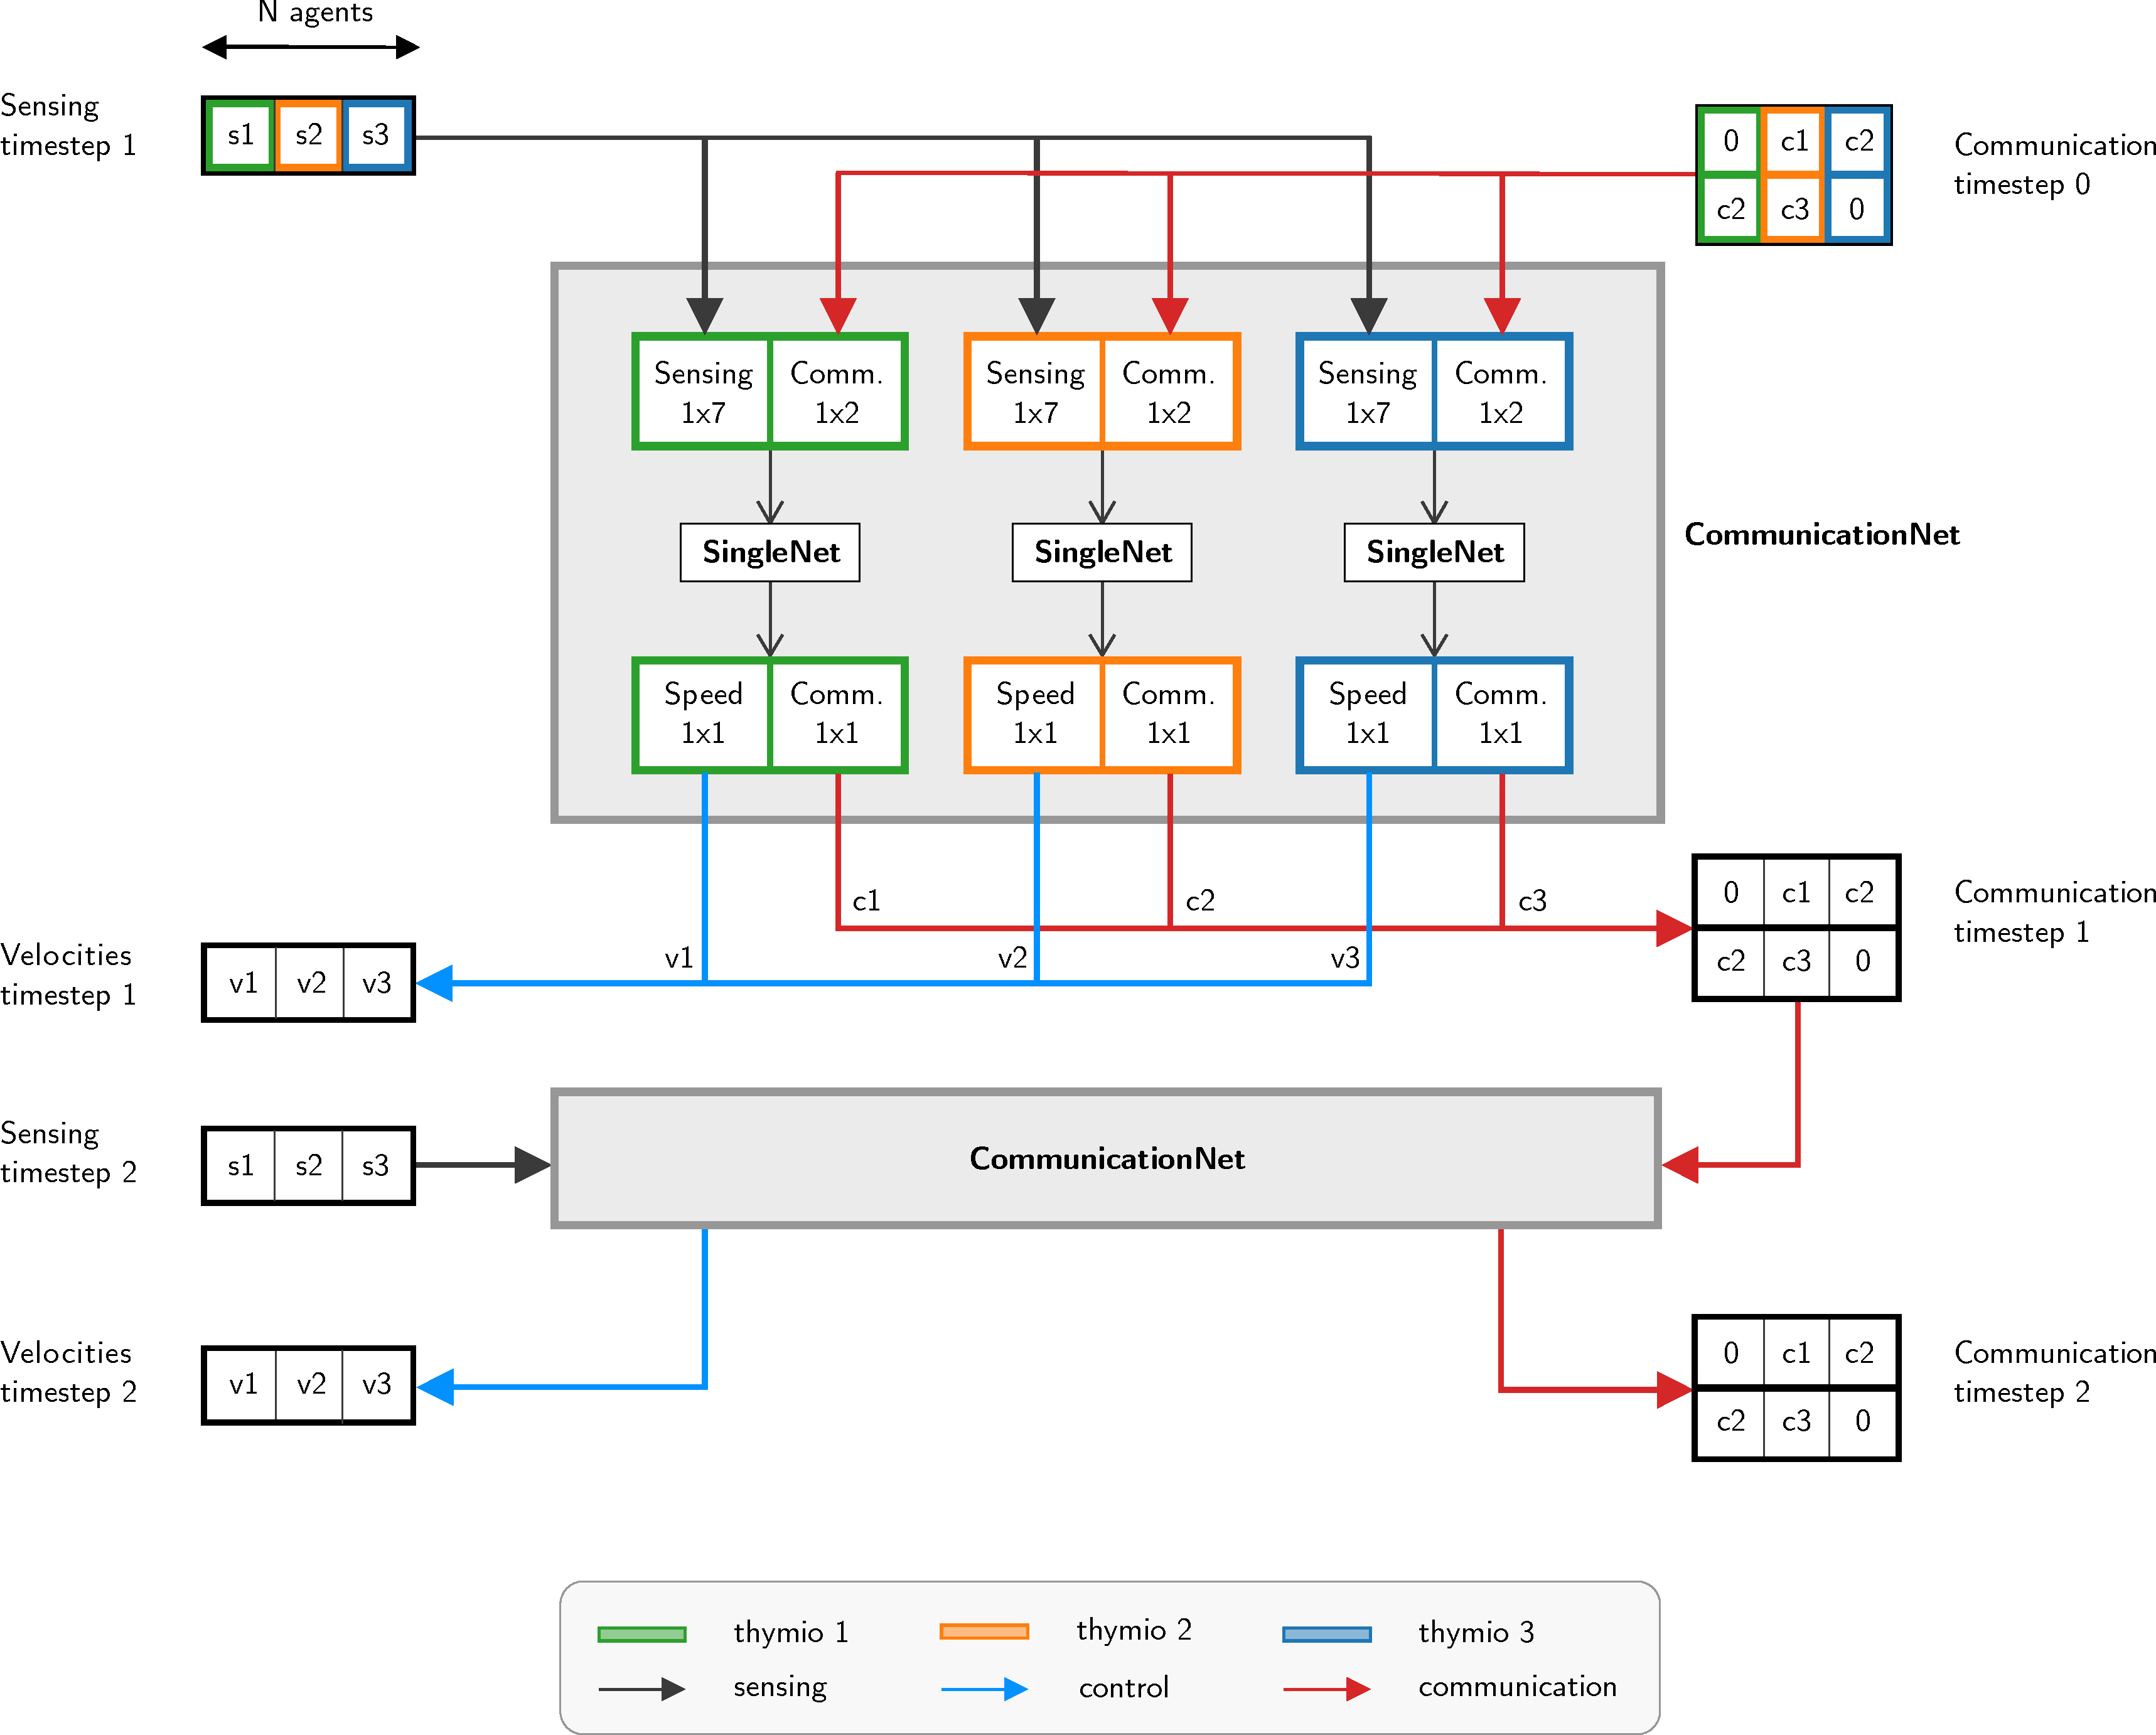
\includegraphics[width=\textwidth]{contents/images/commnet2}
	\caption[Communication network.]{Visualisation of the forward pass of the 
		communication network with three agents and a sequence composed by two 
		timesteps.}
	\label{fig:commnet1}
\end{figure}

The architecture of the \texttt{SingleNet}, displayed in Figure 
\ref{fig:singlenetcomm1}, is almost the same as the one of the distributed 
model without communication: there are three linear layers each of size 
$\langle\mathtt{input\_size} + 2, 10\rangle$,  $\langle 10, 
10\rangle$ and $\langle 10, 2\rangle$, where \texttt{input\_size} is the sum 
of the shape of the sensing and the two communication values received, one 
from the left and one from the right.

\begin{figure}[!htb]
	\centering
	\begin{subfigure}[h]{0.495\textwidth}
		\centering
		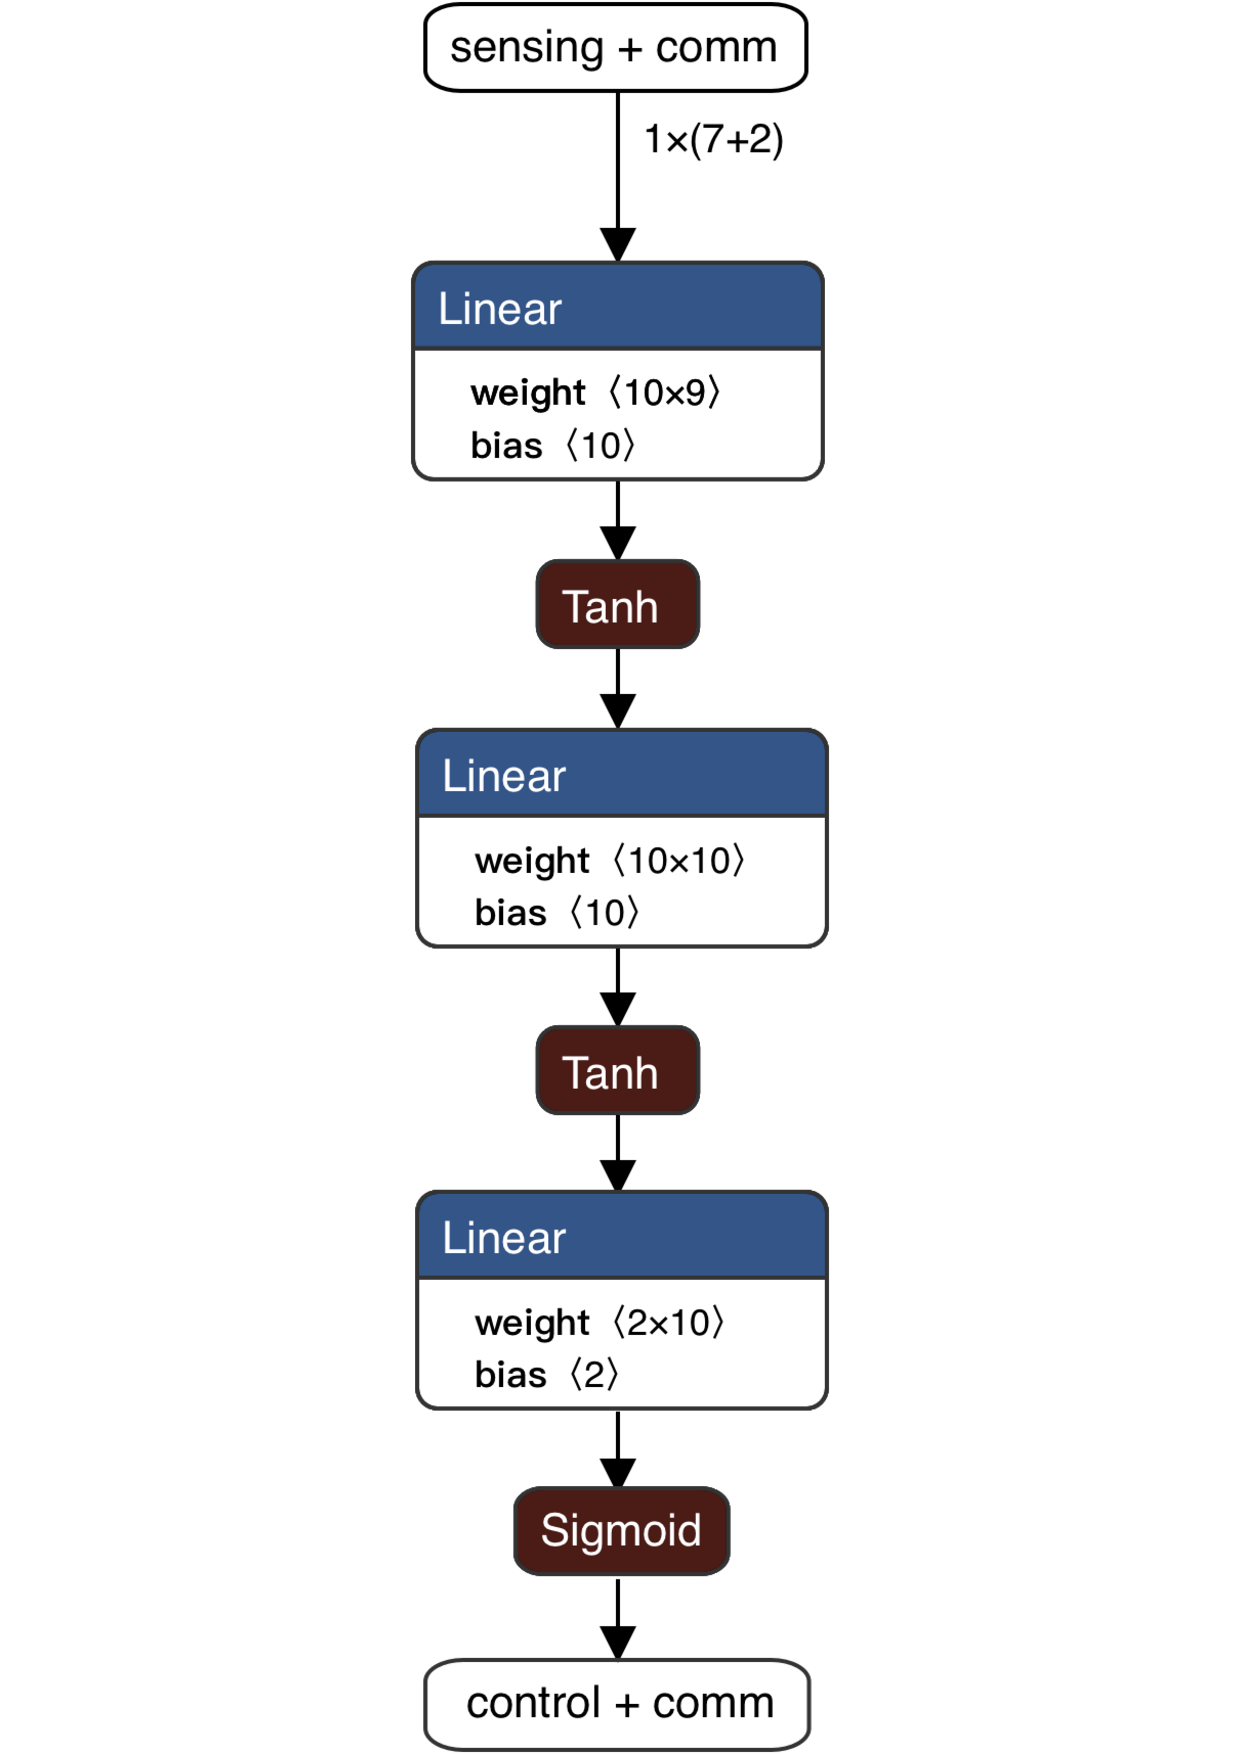
\includegraphics[width=.8\textwidth]{contents/images/task1distributedcomm@4x}%
		\caption{\texttt{SingleNet} with $7$ input sensing.}
	\end{subfigure}
	\hfill
	\begin{subfigure}[h]{0.495\textwidth}
		\centering
		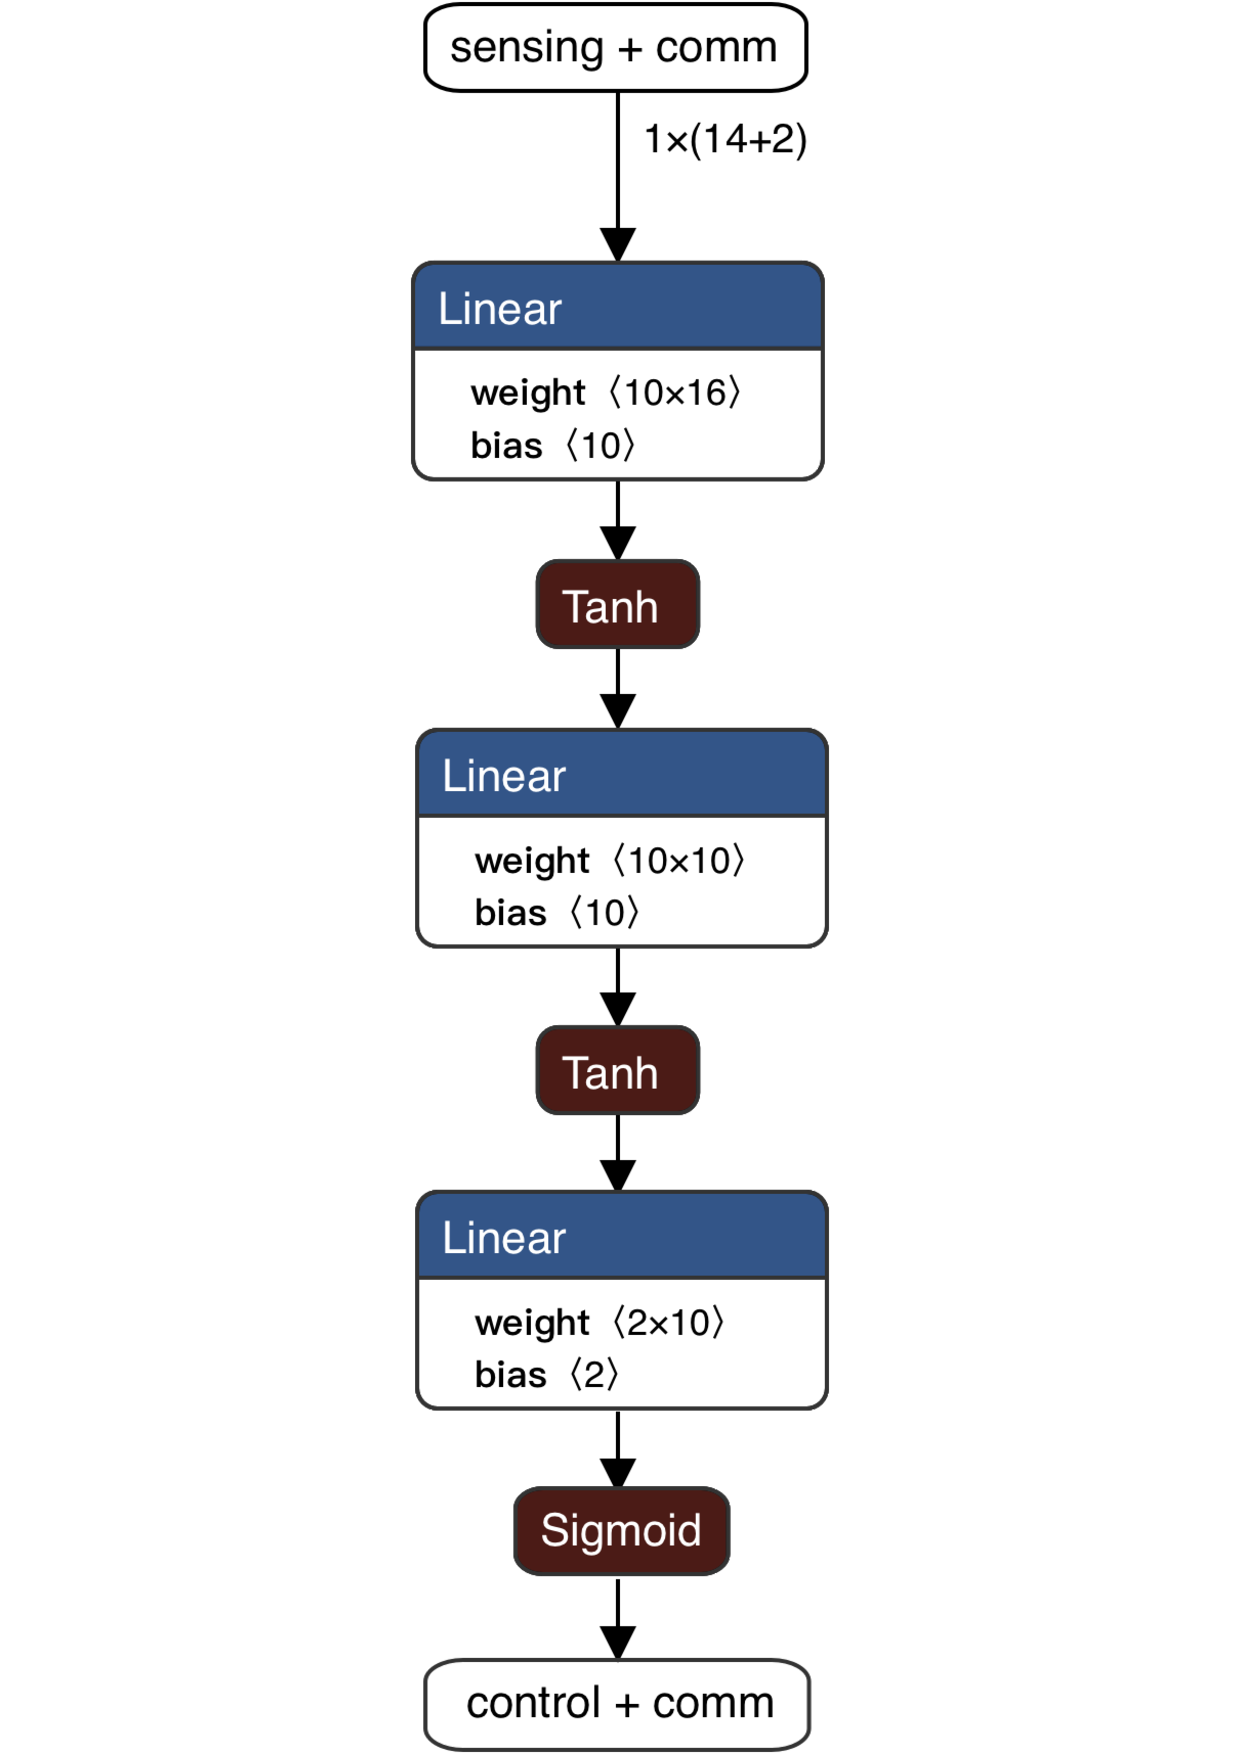
\includegraphics[width=.8\textwidth]{contents/images/task1distributed_allcomm@4x}
		\caption{\texttt{SingleNet} with $14$ input sensing.}
	\end{subfigure}
	\caption[Network architectures for the distributed approach with 
	communication.]{Visualisation of the network architecture chosen for the 
	distributed approach with communication in case of 7 or 14 inputs.}
	\label{fig:singlenetcomm1}
\end{figure}

As before, to the first and second layer is applied a Tanh non-linear 
activation function, while a sigmoid \cite[see][]{han1995influence}, shown in 
Figure \ref{fig:sigmoid}, is applied to the second dimension of the output, 
that is the value of the communication to transmit, in order to normalise it in 
the range $[0, 1]$ and its output is given by
\begin{Equation}[H]
	\centering
	\begin{equation}
	\sigma(x)= \frac{1}{1 + e - x}
	\end{equation}
	\caption{Sigmoid Function.}
	\label{eq:sigmoid}
\end{Equation}

\begin{figure}[!htb]
	\centering
	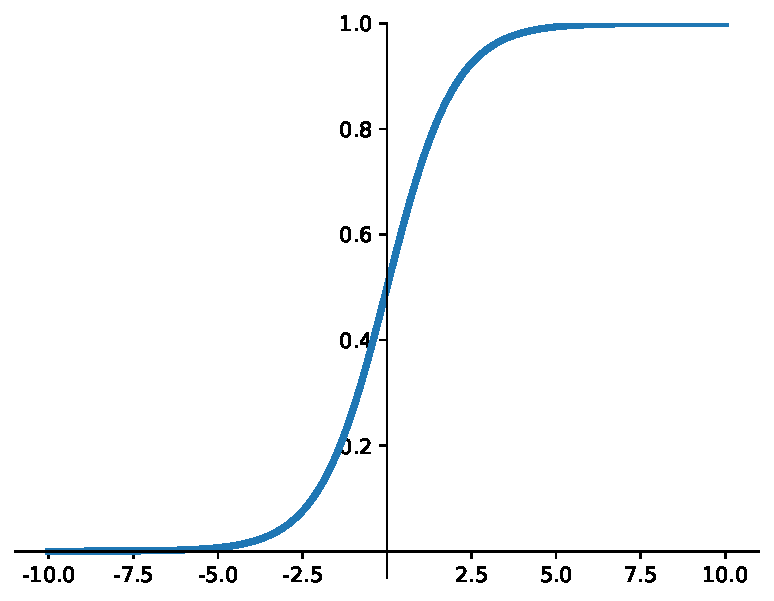
\includegraphics[width=.5\textwidth]{contents/images/sigmoid2}%
	\caption[Trend of the Sigmoid activation function.]{Trend of the Sigmoid 
	Function applied as a non-linear activation to the second output of the 
	network.}
	\label{fig:sigmoid}
\end{figure}

As before, we use Adam optimiser but with a smaller learning rate, $0.001$. 
We split the dataset in mini-batches, this time of size $10$ and then train 
the models for $500$ epochs. 

Finally we evaluate the goodness of the predicted control using the \gls{mse} 
loss function, while the communication is learned in an unsupervised way.
Since the network is fully connected, the communication affects directly the 
output, and consequently, the error minimised, even if it is computed using 
only the control. Improving the loss has an impact also on the 
communication latent variable: since the error is propagated through the 
internal network, in order to update the weight during the back-propagation 
step, that influences the 
communication.

\subsubsection{Experiments}
\label{subsubsec:expcomm}
